%% manuscript produces a one-column, double-spaced document:
\documentclass[manuscript]{aastex}


%\documentclass[twocolumn]{emulateapj}

%% preprint2 produces a double-column, single-spaced document:
%% Sometimes a paper's abstract is too long to fit on the
%% title page in preprint2 mode. When that is the case,
%% use the longabstract style option.

%% \documentclass[preprint2,longabstract]{aastex}

%% If you are submitting to a journal that translates manuscripts
%% into SGML, you need to follow certain guidelines when preparing
%% your macros. See the AASTeX v5.x Author Guide
%% for information.

\newcommand{\vdag}{(v)^\dagger}
\newcommand{\numt}{80}
\newcommand{\cii}{\ensuremath{\mathrm{C}\,\scriptstyle \mathrm{II}}}
\newcommand{\oi}{\ensuremath{\mathrm{O}\,\scriptstyle \mathrm{I}}}
\newcommand{\hi}{\ensuremath{\mathrm{H}\,\scriptstyle \mathrm{I}}}
\newcommand{\heII}{\ensuremath{\mathrm{He}\,\scriptstyle \mathrm{II}}}
\newcommand{\siIV}{\ensuremath{\mathrm{Si}\,\scriptstyle \mathrm{IV}}}
\newcommand{\siIII}{\ensuremath{\mathrm{Si}\,\scriptstyle \mathrm{III}}}
\newcommand{\p}{R$_p$/R$_*$}
\newcommand{\lya}{Lyman-$\alpha$}

%% You can insert a short comment on the title page using the command below.

%%\slugcomment{Not to appear in Nonlearned J., 45.}

%% If you wish, you may supply running head information, although
%% this information may be modified by the editorial offices.
%% The left head contains a list of authors,
%% usually a maximum of three (otherwise use et al.).  The right
%% head is a modified title of up to roughly 44 characters.
%% Running heads will not print in the manuscript style.

\shorttitle{Limb Brightened Transits}
\shortauthors{Schlawin et al.}

%% This is the end of the preamble.  Indicate the beginning of the
%% paper itself with \begin{document}.

\begin{document}

%% LaTeX will automatically break titles if they run longer than
%% one line. However, you may use \\ to force a line break if
%% you desire.

\title{Planetary Transits at Limb Brightened Wavelengths:\\
Detection of Si IV Absorption by HD209458b}

%% Use \author, \affil, and the \and command to format
%% author and affiliation information.
%% Note that \email has replaced the old \authoremail command
%% from AASTeX v4.0. You can use \email to mark an email address
%% anywhere in the paper, not just in the front matter.
%% As in the title, use \\ to force line breaks.

\author{E. Schlawin} 
\affil{Astronomy Department, Cornell University, Ithaca NY 14850}
\author{E. Agol}
\affil{Astronomy Department, University of Washington, Seattle, WA 98195}
\author{J. Lloyd}
\affil{Astronomy Department, Cornell University, Ithaca NY 14850}
\author{L. Walkowicz}
\affil{Astronomy Department,University of California at Berkeley,Berkeley, CA 94720}
\author{K. Covey\altaffilmark{1}}
\affil{Astronomy Department, Cornell University, Ithaca NY 14850}


%%\affil{Astronomy Department, Cornell University,
%%    Ithaca, NY 14853}

% PUT THIS BACK IN ONC YOU FIGURE OUT HOW TO MAKE IT NOT CONFLICT WITH TEXT
%\altaffiltext{1}{Hubble Fellow}

%% Mark off your abstract in the ``abstract'' environment. In the manuscript
%% style, abstract will output a Received/Accepted line after the
%% title and affiliation information. No date will appear since the author
%% does not have this information. The dates will be filled in by the
%% editorial office after submission.

\bibliographystyle{apj}

\begin{abstract}
Observations of extrasolar planetary transits are valuable tools for measuring planetary radii and  constraining the structure and chemical composition of planetary atmospheres. For most of these observations, transit light curves have only one minimum and a  ``U'' shape. However, for optically thin chromospheric emission lines, stars appear strongly limb-brightened so their light curves have two minima and hence, a ``W'' shape. In this Letter, we calculate theoretical transit light curves for limb brightened wavelengths and fit these models to the \siIV\ emission line in HD209458b. We find that the best fit \siIV\ absorption model has R$_{p,\siIV}$/R$_*$ = 0.34 $\pm$ 0.15, similar to the Roche lobe of the planet.
\end{abstract}

%% Keywords should appear after the \end{abstract} command. The uncommented
%% example has been keyed in ApJ style. See the instructions to authors
%% for the journal to which you are submitting your paper to determine
%% what keyword punctuation is appropriate.

\keywords{extrasolar planets: transit detections -- stellar chromospheres -- HD209458b}
%% Authors who wish to have the most important objects in their paper
%% linked in the electronic edition to a data center may do so by tagging
%% their objects with \objectname{} or \object{}.  Each macro takes the
%% object name as its required argument. The optional, square-bracket 
%% argument should be used in cases where the data center identification
%% differs from what is to be printed in the paper.  The text appearing 
%% in curly braces is what will appear in print in the published paper. 
%% If the object name is recognized by the data centers, it will be linked
%% in the electronic edition to the object data available at the data centers  
%%
%% Note that for sources with brackets in their names, e.g. [WEG2004] 14h-090,
%% the brackets must be escaped with backslashes when used in the first
%% square-bracket argument, for instance, \object[\[WEG2004\] 14h-090]{90}).
%%  Otherwise, LaTeX will issue an error. 

\section{Introduction}
Of the exoplanets so far discovered, more than \numt\ are known to
transit their host star (\texttt{www.exoplanet.eu}) . Transits cause observable effects that can constrain exoplanetary composition and size, and accurate timing of transits can reveal when their orbits are perturbed by other bodies \citep{winnchap}. When these transits are observed in the ultraviolet, they show much deeper transits than for visible wavelengths, revealing that atmospheres extend far beyond the optical radius of planets \citep{vidmad,benjaf7,mclay,lecav,fossati}. Ultraviolet measurements also constrain atmospheric conditions and how much mass is escaping the planet's Roche lobe \citep{knutsonprop,gmunoz,linsky}.

For most transit light curves, the overall brightness of the system is at a minimum when the planet crosses the sub-earth longitude of the star (phase = 0.0). Depending on the extent of stellar limb darkening, the bottom of the light curve can be flat or curved concave up. This occurs with uniform stellar emission across the disk and limb darkening, respectively.
% Even more information about their orbit can be gleaned from
%the exact epoch at which they transit their host star. So called
%transit timing variation (TTV) measurements
%\citep{2005MNRAS.359..567A} (and cite more?) are designed to reveal
%deviations from Keplerian elliptical motion due to the tug other
%planets and satellites.
%
%Previous transit timing has been done with optical and infrared
%telescopes \citep{2004ApJ...613L.153A,2010A&A...510A.107M} (\& add
%some more TTV papers?) Light curves for these kind of transits have a
%sharp negative slope at ingress and a sharp positive slope at
%regress. In the middle, they have a gradual concave up curvature due to limb darkening of the star.

\citet{assef} point out that observations of emission lines that show strong limb brightening instead have {\it two} minima; some
wavelengths are limb brightened so the flux at these wavelengths goes
{\it up} mid-transit and to a minimum at each stellar limb. This occurs for all optically thin
chromospheric or coronal emission lines because they show strong limb brightening. Just as with a planetary
nebula, like the Ring Nebula, the limb of an optically thin shell of
gas is brighter at the edges. This is because the column density is much larger at the limb than in the center and because the photospheric emission beneath the chromosphere is negligible.\footnote{Note
that this effect is different from what causes limb darkening.} As a
consequence, such a transit curve will be ``W''-shaped, where the maximum
transit depth occurs at the stellar limbs.

\citet{assef} point out that limb brightening could be
useful for detection of transits of planets orbiting giant stars. One advantage
to photometry in limb brightened wavelengths is that transits are
deeper overall than for both limb darkened and uniform disk
emission. This is because the star emits over a smaller effective area--a ring instead of a disk--so the planet covers a larger amount of the
stellar flux. \citet{assef} approximate the limb brightened
star as a uniform ring of emission. With their approximation, the maximum depth
of the transit is  $\propto R_p/R_*$ instead of $(R_p/R_*)^2$,
as expected for a uniform disk. This is because the planet covers $\sim$2R$_p$ out of a circle of emission whose total circumference is 2$\pi$R. 

We present in this paper a slightly more detailed model of optically thin stellar emission that includes flux from the central region of the stellar disk. Under this model, the maximum transit depth scales as $(R_p/R_*)^{3/2}$, instead of $R_p/R_*$. In
$\mathsection$\ref{labl:chromlcurve} we calculate the expected limb
brightened light curve for an optically thin emission line. We
compare this model UV light curve with \siIV\ emission from HD209458b in  $\mathsection$\ref{osiris} and discuss the implications for HD209458b's exosphere in $\mathsection$\ref{discuss}.

\section{A Limb Brightened Curve Under The Thin-Shell Approximation} \label{labl:chromlcurve}
\label{labl:thinshell}

For optically thin emission, the total flux from the chromosphere is proportional to the total number of emitting species. If the emitting species are distributed with a uniform density, then the total flux is proportional to the volume of the chromosphere. We make the approximation that the scale-height of emission, $h$, is much smaller than the size of the planet ($R_p$) and star ($R_*$).

Under this geometrically thin approximation, the total flux from the star is proportional to the surface area of the hemisphere facing the Earth, as pictured in Figure \ref{fig01}, times its thickness $h$. The amount of emission that the planet blocks is then simply the amount of the stellar surface that the planet covers times $h$. In this geometrical limit, therefore, the scale height of the chromosphere cancels out.

%then we can treat the
%chromosphere as a geometrically thin hemisphere of emission.  This
%limit has the problem that at the edge of the shell, the surface
%brightness will be infinite.
%; this is an example classic fold-caustic.
%However, when one integrates the surface brightness over area, the
%total flux is finite, and thus this still proves to be a useful
%approximation.

%However, rather than integrating over surface brightness to compute
%the transit depth, 
%the depth of transit is simply the area of the 
%hemisphere that is blocked by the planet, 

We can estimate the maximum depth of transit as follows from
Figure \ref{fig01} by comparing the total emitting area of the star to the total stellar surface area blocked by the planet. The blocked surface is the same as the shadow produced by a sphere of radius $R_p$ onto a hemisphere of radius $R_*$. When the planet touches the edge of the star 
(second contact), as shown from an edge-on viewpoint in this figure,
then the length of the arc of the long axis of the shadow is
$R_*\theta$.  The diameter of the planet is 
$2 R_p \approx R_*(1-\cos{\theta}) \approx \frac{1}{2} R_* \theta^2$,
where the latter approximation is valid for $\theta \ll 1$.
Solving for $\theta$, we find $\theta = 2\sqrt{R_p/R_*}$, so to
be valid we require $R_p/R_* \ll 1/4$.  We can approximate
the shadow as an ellipse which will have a semi-minor axis of $R_p$
and a semi-major axis of $R_*\theta$, so we can approximate the
area of the shadow as $A_t = \pi \sqrt{R_pR_*} R_p$.  Thus,
the maximum depth of transit is given by 
\begin{equation} \label{depth_anal}
\delta_{\mathrm{max}} = {A_t \over 2 \pi R_*^2} = \frac{1}{2} \left({R_p \over R_*}\right)^{3/2}
\end{equation}
Note that this is a different scaling than that given in \citet{assef} who assume that there is no emission from the central region of the star. The qualitative difference is pictured in Figure \ref{limbmodel}.

%Koskinen et a. 2010 treat \oi emission as two separate pieces - limb and disk. Maybe this is OK if OI emission is optically thick

This has the remarkable consequence that the depth of a chromospheric
transit does not decline as much with the radius of the planet as 
a transit of a uniform disk.  A chromospheric transit has a maximum
depth that is $\frac{1}{2} \left({R_* \over R_p}\right)^{1/2}$
times deeper than the maximum transit depth of a uniform disk;
thus smaller planets have an advantage to be observed at
chromospheric wavelengths, as emphasized by \citet{assef}. It should also be noted that most limb brightened lines are in the ultraviolet, where planets absorb light from a larger radius than for optical and infrared wavelengths \citep{vidmad}. This means that maximum transit depths of ultraviolet emission lines are enhanced {\it doubly} over optical emission, once for the (\p )$^{1/2}$ scaling and once for the additional atmospheric absorption.

\begin{figure}
%\centerline{\psfig{figure=Chromospheric_shadow.eps,width=4in}}
%\includegraphics[trim = 1in 6in 2in 0.5in,clip,width=3
%  in]{Chromospheric_shadow.eps}
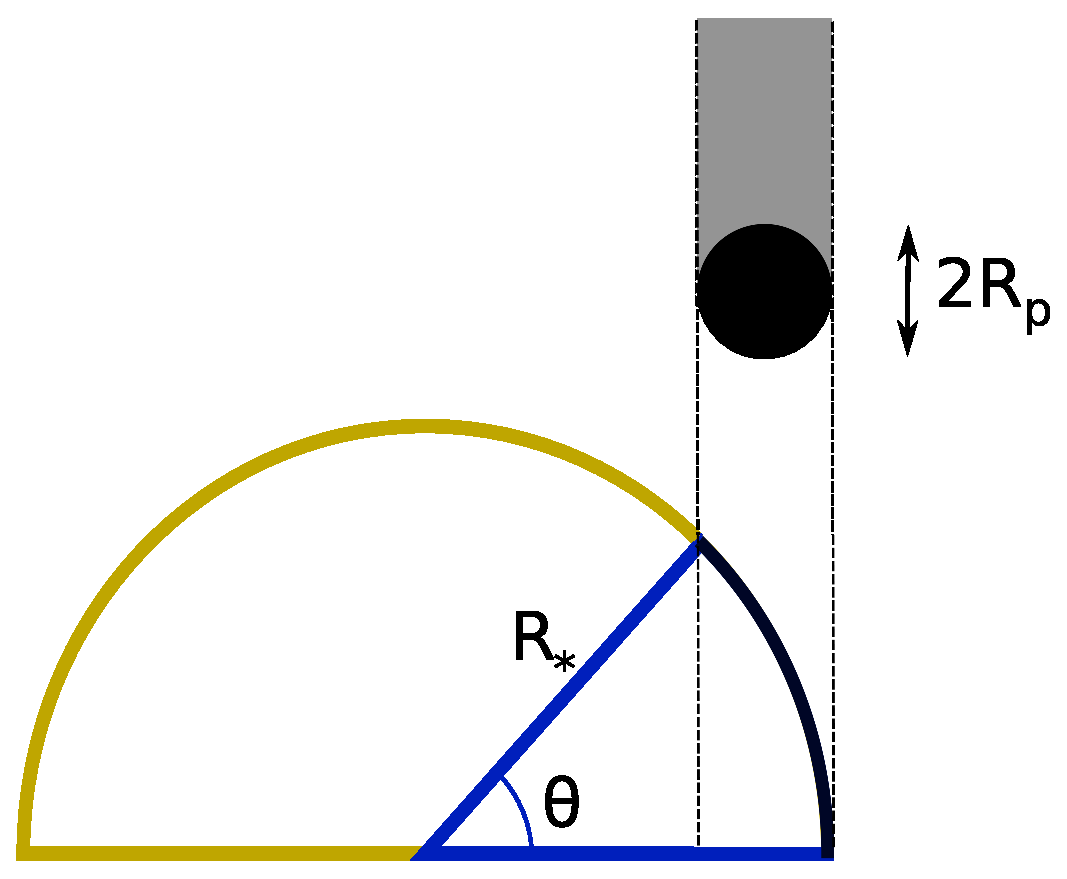
\includegraphics[width=0.5 \textwidth]{chrom_shadow2.eps}
\caption{Edge-on view of area of stellar emission and the amount blocked by  a planet. This blocked surface area is the same as the area of a shadow cast by a sphere onto a hemisphere.}
\label{fig01}
\end{figure}

We can compute the light curve for a negligible scale height ($h=0$) by finding the area of the the planet's shadow and dividing this by the surface area of a hemisphere with radius $R_*$. The volume of the intersection of a cylinder with a sphere is given by \citet{lamarche} and we find the surface area of the intersection by taking a partial derivative with respect to radius. The result can expressed analytically in terms of elliptic integrals.
Let $x$ be the distance, in units of stellar radii $R_*$, from the center of the planet to the center of the star projected onto a plane perpendicular to the observer. To calculate the light curve for a planet that does not pass through the center of the star, one can simply write $x(t)$ as $\sqrt{t^2+b^2}$, where $t$ is the distance to the closest approach point in stellar radii $R_*$ and $b$ is the impact parameter (the planet-star distance at closest approach) in stellar radii $R_*$. 
%Let $b$ be the impact parameter of center of the planet relative to
%the center of the star in units of the radius of the star, as
%seen by an observer. 
%Let $a = A_t/R_*^2$ be the dimensionless transit
%area, and $f(b,p)=1-\frac{a}{2\pi}$ is the transit light curve.

The transit depth, $\delta (x)$ is split up into three different regimes: $0 < x < 1 -p$, $1 - p < x < 1+p$ and $ 1+p < x$. The transit depth, $\delta (x)$ = 0 when $x > 1 + p$ since no emission is blocked by the planet.
For $1-p < x < 1+p$, the planet straddles the edge of the star, and
 for $0 < x < 1-p$, the planet is fully contained within the disk of the star. The transit depth is 
% Explicitly,
%\begin{eqnarray}\label{ellipint}
%K(m)&=&\int^1_0 {dz \over \sqrt{1-z^2}\sqrt{1-m z^2}}, \cr
%E(m)&=&\int^1_0 {dz \sqrt{1-z^2} \over \sqrt{1-m z^2} }, \cr
%\Pi(n;K(m)|m)&=&\int^1_0 {dz \over \left( 1-n z^2 \right) \sqrt{1-z^2} \sqrt{1-m z^2} }
%\end{eqnarray}

\begin{eqnarray}\label{disk}
\delta(x)&=& \Theta (p-x)+\frac{a_0}{2 \pi \sqrt{xp}} \times \\
&&\left[\frac{x+p}{x-p} \Pi(n,m) - 4 x p a_1 E(m) - a_2 K(m) \right] \nonumber
\end{eqnarray}

\begin{table}[htdp]
%\caption{default}
\begin{center}
\begin{tabular}{c c c c}
 & $0 \le x \le 1-p $& $1 - p < x \le 1+p $&$ 1+p < x $ \\
$a_0$ & $\sqrt{m} $& 1 & 0\\
$a_1$ &$ \frac{1}{m} $& 1 & \\
$a_2$ & $p^2-x^2 $& 1-2p(x+p) & \\
m & $4xp\over 1-(x-p)^2$ & $\frac{1-(x-p)^2}{4xp}$$ $& \\
n & $-4xp/(x-p)^2$ & $1-(x-p)^{-2}$ & $$
\end{tabular}
\end{center}
\label{default}
\end{table}%
where $K(m)$, $E(m)$, and $\Pi(n,m)$ are complete Legendre elliptic 
integrals of the first, second, and third kinds, and $\Theta(x)$ is
the Heaviside step function. For the elliptic integrals, we use the conventions of \citet{handbk} where $\Pi(n,m) = \Pi(n;K(m)|m)$ for the third elliptic integral.



These formulae are difficult to evaluate numerically at 
$x=p$ and $x=1-p$ due to the divergenced of $K(1)$ and $\Pi(n,1)$
; the divergences cancel out analytically, but routines that
evaluate the elliptic integrals diverge.  However, these locations
are a set of measure zero, and thus should almost never be encountered
when modeling data.

%\subsection{Dependence on planet size}

Figure \ref{fig02} (solid curve) shows the transit light curve (1-$\delta (x)$) for a planet that has \p =0.08 using a thin-shell approximation.  The analytic estimate given by equation \ref{depth_anal} and the more detailed equation \ref{disk} agree well, predicting maximum chromospheric depths to be 1.8 times
deeper than for uniform disk brightness.\footnote{For a uniform disk emission $\delta_{\mathrm{max}} $=$\pi R_p^2 /(\pi R_*^2)$.} 
%Although the smaller
%planet has a transit depth that is 25\% of the larger planet's
%transit depth for a star without limb-darkening, the maximum 
%chromospheric transit depth for the smaller planet is 35\% that 
%of the larger planet, and is nearly as deep as the transit of 
%the larger planet.  Note that the duration of ingress/egress 
%scales with the size of the planet in both cases.  

%There are two consequences of the deeper transit depth:
%(1) the larger depth and short duration
%of the chromospheric transit can make detection of giant
%planets transiting sub-giant stars greater possibility, as emphasized by \citet{assef}
%and (2) since the advantage of chromospheric transits
%over continuum transits grows as $\frac{1}{2}p^{-1/2}$,
%the chromospheric transits have a greater advantage for
%transit detection of small planets. For instance,
%for $p=0.01$, the chromospheric transit is $5\times$
%deeper, which is appropriate for Earth-Sun transits
%or giant planets transiting a $10R_\odot$ star. The transit will be even deeper if the planet's atmosphere extends beyond the visible radius.

%Although the considerations in this section apply
%for the geometrically-thin shell approximation,
%we now show that this also applies when one considers
%the physical extent of the chromosphere.

\begin{figure}
%\centerline{\psfig{figure=comp_size.eps,width=4in}}                            
%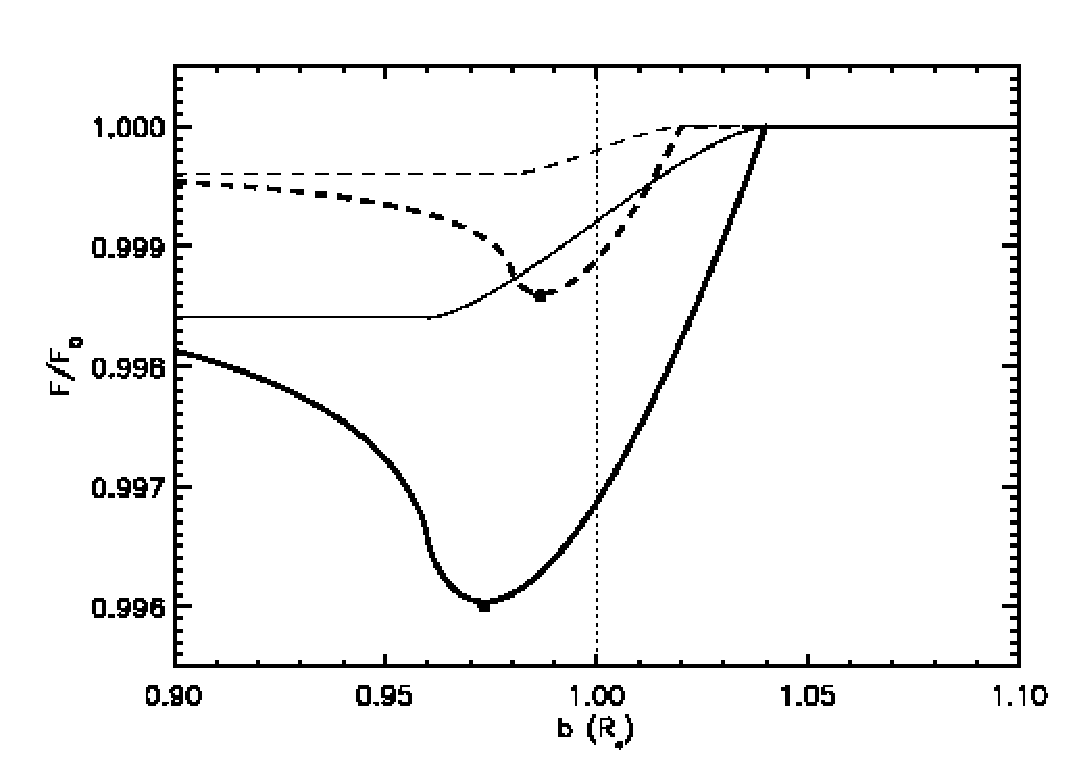
\includegraphics[trim = 1in 6in 2in 0.5in,clip,width=3                         
%  in]{comp_size.eps}                                                           
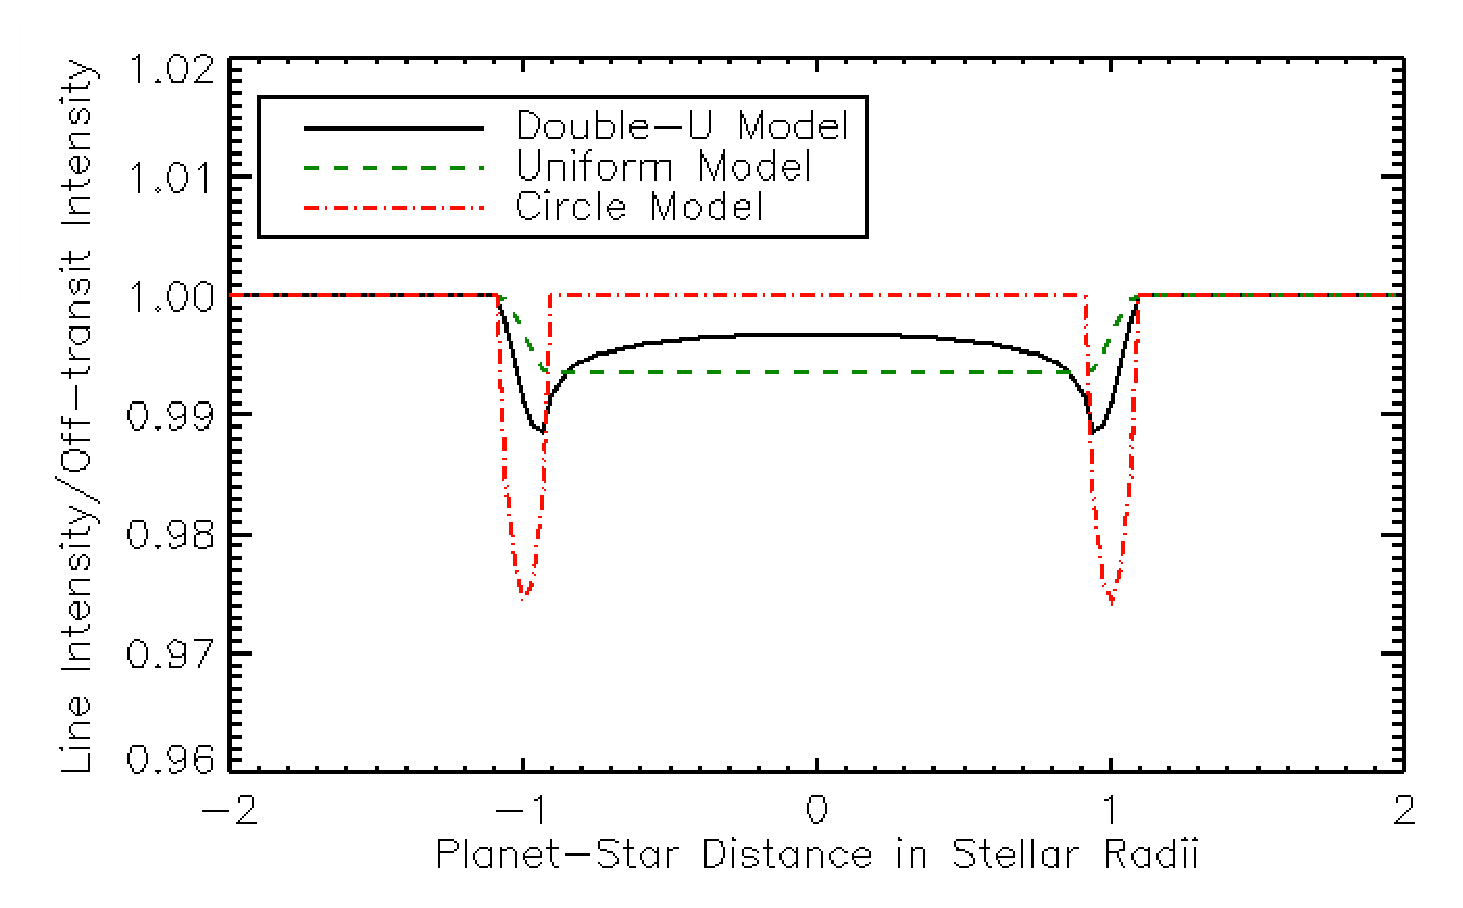
\includegraphics[width=0.5 \textwidth]{model_compare2.eps}
\caption{Transit light curve for \p $=0.08$, using a family of 3 different models. The solid line is a Double-U model, using equation \ref{disk}. The Uniform model (dashed line) is one for which the emission is assumed to be constant across the stellar disk. The dot-dash line is a model where the emission is assumed to be only from the limb as pictured in Figure \ref{limbmodel}. Note that the Double-U models' minima are deeper than the uniform emission model and that these minima occur at the stellar limbs. }
\label{fig02}
\end{figure}


\begin{figure}
\begin{center}
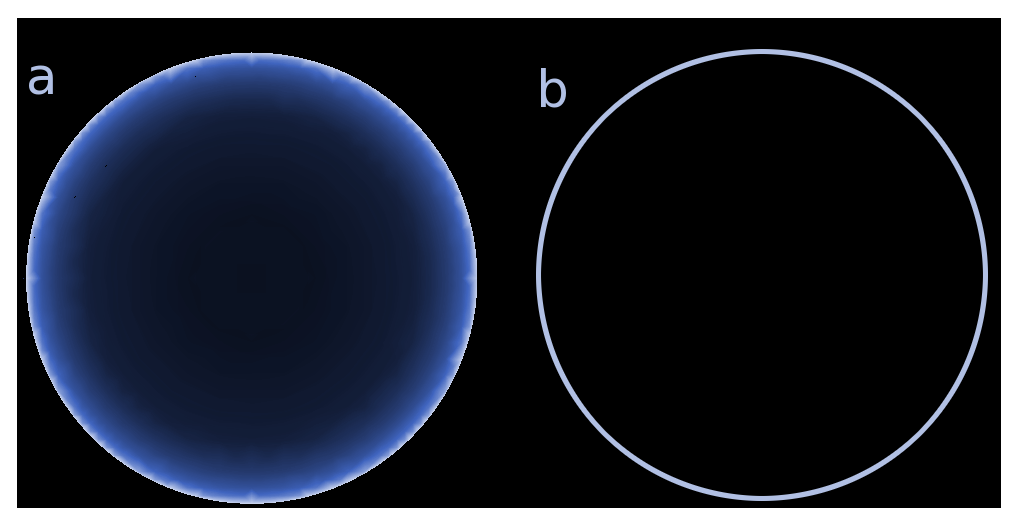
\includegraphics[width=0.5\textwidth]{model_comparison.eps}
\caption{Model Limb Brightening. (a) A model of spherically symmetric optically thin emission includes some emission from the central parts of the star. (b) An approximate model where all the emission is from the stellar limb. We employ the model shown in (a) for \siIV\ emission, and whose light curve is given by  equation \ref{disk}.}
\label{limbmodel}
\end{center}
\end{figure}

\begin{figure}
\begin{center}
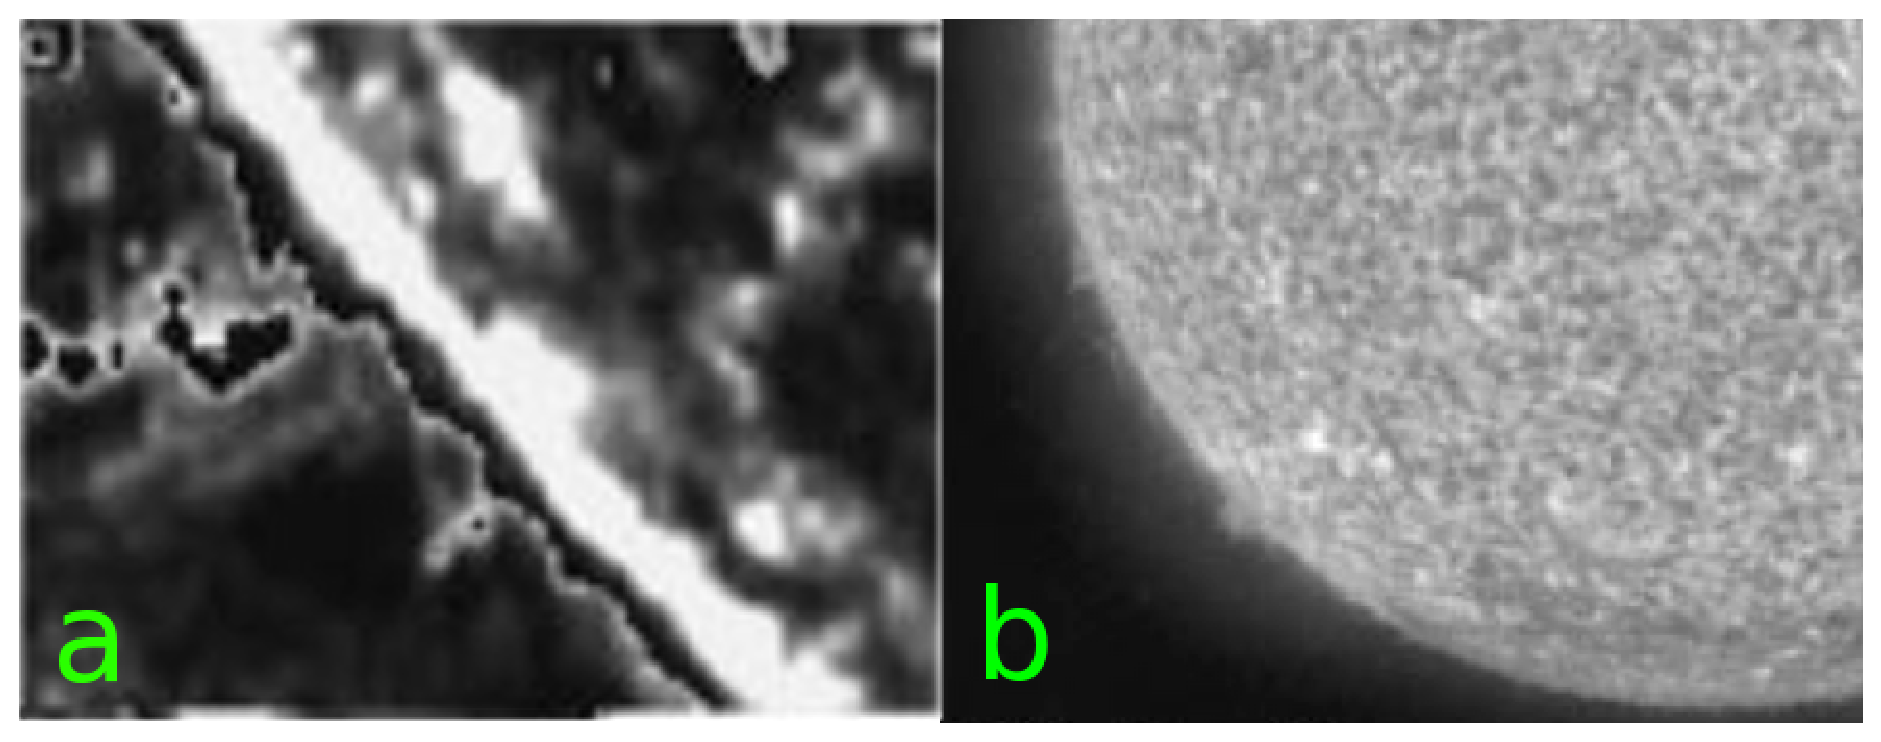
\includegraphics[width=0.5\textwidth]{limb_compare_siIV_heII.eps}
\caption{(a) \siIV\ emission from the Solar limb as observed by SUMER (Solar Ultraviolet Measurement of Emitted Radiation) \citep{wiik} is strongly limb-brightened, indicating that a transit of this emission line should have a Double-U light curve. (b) \heII\ 304 \AA\ image of the solar limb, taken by the Extreme-ultraviolet Imaging Telescope \citep{feldman} is, by contrast, not limb brightened because it is optically thick in the chromosphere and thus the additional column density at the limb does not contribute any more flux then the central disk.}
\label{limbs}
\end{center}
\end{figure}

\section{\siIV\ Absorption by HD 209458b} \label{osiris}

\citet{viddisc} observed HD 209458b with the Hubble STIS instrument and found
an extended Hydrogen, Oxygen and Carbon atmosphere by fitting the light curves
to the near-UV \hi\, \oi\ and \cii\ lines during a transit. They found no absorption in \siIV\ when trying to fit the light curve to a model of a spherical planet occulting a {\it uniform} stellar disk.

We fit their \siIV\ 1394 \AA\ data (\citet{vidmad}, Figure 3) with a Double-U model given by equation \ref{disk}. This model is appropriate for the \siIV\ emission, as evident in the Solar image in Figure \ref{limbs} (a) where strong limb-brightening is apparent; we assume that HD209458 is also limb-brightened because it is a G0V star, close to the Solar type.

The best fit model has two free parameters: the planet/star radius ratio \p\ and an overall constant that sets the off transit-flux. The second parameter is necessary since the off-transit flux is poorly constrained. The impact parameter 
%described in $\mathsection$\ref{labl:thinshell}
 is fixed for the model. We adopt a value of $ b= 0.48 R_*$, using the an inclination of 86.9$^\circ$ \citep{knutsonprop} and a semi-major axis $a=8.82 R_*$.

Figure 5
%\ref{lightc} !!!!!!!!! Why doesn't this ref{} work properly It says 3!!.
 shows the light curve for \citet{vidmad}'s data and the best fit model. In addition to the best fit model, we show three more limb brightened models where \p\ is a fixed parameter for comparison. These include \p\ equal to 0, 0.12, and 0.32 representing no \siIV\ absorption, the optical radius \citep{knutsonprop} and the \hi\ radius\footnote{This was found by \citet{vidmad} for absorption of the wings of the \lya\ emission profile}, respectively.

Using a Levenberg-Marquardt fitting algorithm \citep{mpfit}, we find that \p\ = 0.34 $\pm$ 0.15. 
The Double-U model has a total $\chi^2$ 3.1 less that fitting the data to
a horizontal line (representing no detection), where the Double-U model has 10 degrees of freedom and the horizontal line has 11. This best-fit model has
R$_p$/R$_*$ = 0.34, close to the 0.32 found by \citet{vidmad} for the narrowband \lya\ detection, representing absorption of \siIV\ by a Roche Lobe-sized atmosphere. Both the Bayesian Information Criterion and Akaike Information Criterion favor the Double U model, even though they punish additional parameters more strongly. The BIC for a Double U model is -16.3 and is -14.9 for the horizontal line model.

%Additional d
%re-analysis of this data for more optically thin lines could improve
%the confidence levels of the fit.

\begin{figure}[!ht]
\begin{center}
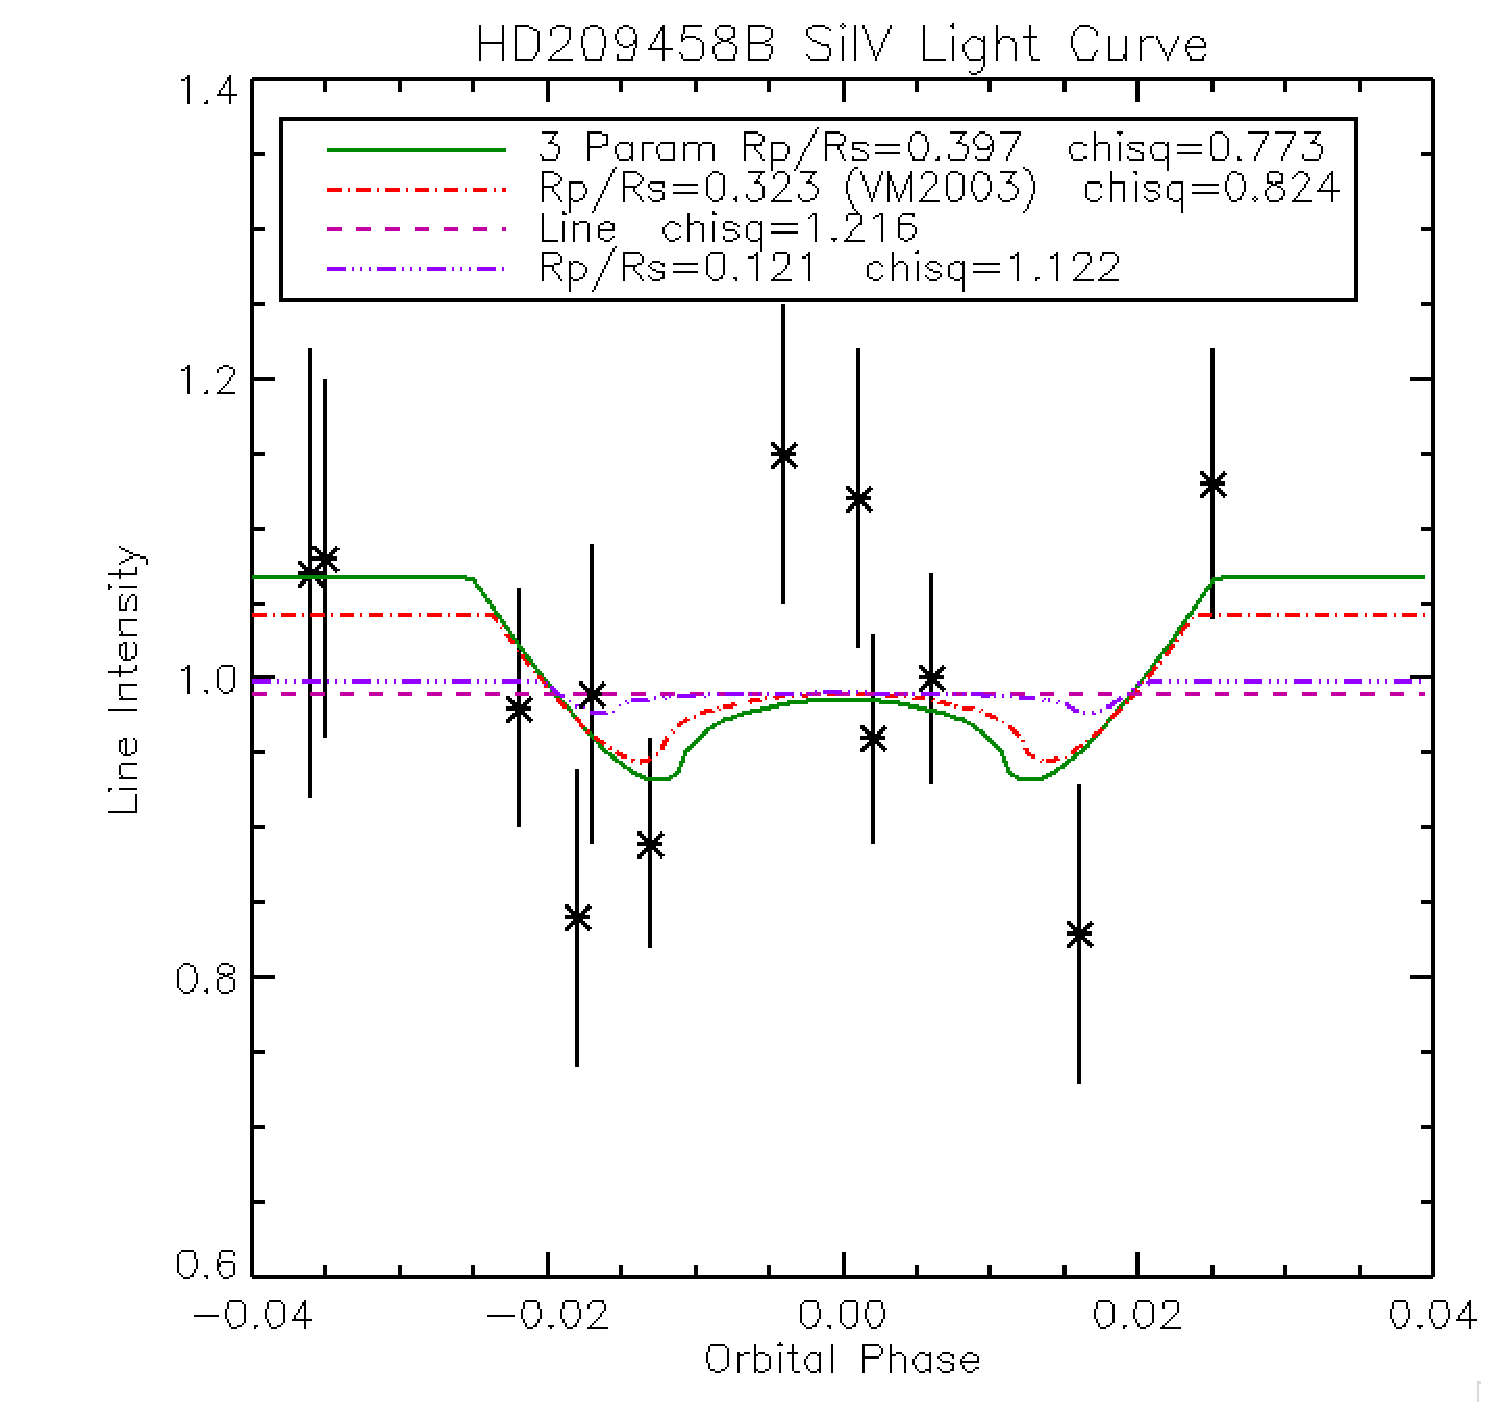
\includegraphics[width=0.5 \textwidth]{hd209458.eps}
\caption{The light curve of the limb-brightened chromospheric line \siIV\ during the transit of HD209458b, as taken by \citet{vidmad} for a wavelength range of [1391 \AA,1397 \AA]. Most of the emission in this range is dominated by the \siIV\ and not contiuum, so we assume entirely optically thin emission from the star. The solid line is a best fit model, using equation \ref{disk} where the radius is a free parameter. For reference, three different best-fit models are shown where the planet size is a fixed parameter: the dash dotted line has a R$_p$/R$_*$ = 0.323 as found by \citet{vidmad} for the Lyman-$\alpha$ absorption. The dashed curve is a horizontal line, corresponding to R$_p$/R$_*$ = 0 or a non-detection of \siIV\ absorption. The dash triple-dotted line is a model with a visible radius, R$_p$/R$_*$ = 0.323. All models have 1 free parameter that is an overall multiplier that sets the off-transit flux. The best-fit radius with R$_p$/R$_*$=0.323 and a normalized $\chi^2$ of 1.04 is close to the model with the radius found by \citet{vidmad}, which indicates \siIV\ absorption from a Roche lobe-sized cloud. }
\end{center}
\label{lightc}
\end{figure}

\section{Discussion} \label{discuss}

Limb brightening has important effects on transit light curves, especially when considering optically thin emission lines from the star. The Double-U model for the \siIV\ transit fits the data better than a non-detection, even when accounting for the additional degrees of freedom in the model. The best fit model gives a \siIV\ transit depth of 11$^{+9}_{-6}$\% at the limb  of the star, which requires a layer of Si$^{3+}$ as large or even larger than the planet's Roche lobe.

The \siIV\ transit depth is comparable to the \oi\ transit depth calculated by \citet{vidmad} and the \hi\ transit depth calculated by \citet{benjaf7}. As \citet{kosk} point out, a hard sphere, which we assume in equation \ref{disk}, is a poor approximation to atmospheric absorption. The \siIV\ absorption profile, instead of having a sharp transition from opaque to transparent, should changes smoothly from optically thick to optically thin absorption in a more accurate model. In order to explain the large transit depth, this smooth model would have to have a radius extending beyond the planet's Roche lobe, R$_{Roche}$/R$_*$ = 0.35 \citep{ben10} to explain the observed transit depth.

The best-fit transit depth supports models with high concentrations of metallic ions in the atmosphere because the radius of \siIV\ absorption is as large as for \hi\ absorption. \citet{kosk} point out that if the metallicity is high, the temperature must also be elevated. The $\approx$ 10,000 K temperature suggested by \citet{gmunoz}, \citet{mclay}, and \citet{kosk} for the thermosphere may not explain large abundances of Si$^{3+}$ needed for the observed absorption. 

% substantial mass flow from the planet onto the star? It is also possible that the \lya\ absorption and \siIV\ absorption come from different regions--\lya\ coming from ~3 R_p and \siIV\ from even higher up

\citet{linsky}, like \citet{vidmad} find no \siIV\ absorption by HD209458b. They did not generate a full light curve, however, and only observed \siIV\ mid-transit. It should be noted that for zero impact parameter, the mid-transit Double-U flux is $\approx 0.5 $(\p)$^2$ because the planet shadow is $\approx \pi {R_p}^2$ and the hemisphere has an area of 2$\pi {R_p}^2$. With the impact parameter of 0.477 (see $\mathsection$\ref{osiris}), we expect the mid-transit depth to be  7$^{+9}_{-5}$\%. 

\citet{linsky} point out that the amount of Si$^{2+}$ may vary appreciably over short timescales because of change in stellar wind speed, planetary mass-loss rate or temperature changes. They observed significant \siIII\ absorption at the same epoch in which they see no \siIV. If \siIV\ is truly not in the absorption spectrum, then there could have been a change in ionization state from Si$^{3+}$ to Si$^{2+}$. The absorption features found at +20 and +40km/s in their spectrum could be some Silicon still in the Si$^{3+}$ ionization state.

Additional observations will help confirm or refute the detection of \siIV\ at the limb of HD209458b and also put further constraints on the system. With enough signal to noise, the light curve may reveal asymmetries in the transit having to do with asymmetric spatial distribution of the UV-absorbing cloud. The advantage of the limb brightened emission lines is that they come from a smaller spatial area of the star and therefore probe the spatial distribution of the planetary atmosphere better than optically thick emission. Accurate time resolved transit data may also reveal differences in {\it thermal} properties of the leading and trailing sides of the planet as predicted by \citet{fortney}.

\section{Conclusion}

Optically thin emission lines produce qualitatively different transit light curves than optically thick emission lines. The maximum transit depths at optically thin wavelengths is $\approx$ 0.5 (\p )$^{3/2}$ whereas thick ones have depths $\approx$ (\p )$^2$. The consequence of this scaling is that small planets will have larger transit depths in thin emission lines than thick lines. There is already an enhancement of UV lines over optical photometry due  to planets' extended atmosphere occulting more of the star than the optical radius \citep{kosk}, so the enhancement of transit depth for optically thin emission boosted doubly over optical measurements.

The best time to observe these optically thin emission lines is when a planet crosses its host's limb and not at a phase of 0, since the Double-U curve is deepest at the stellar limb. Observations at the limb have a depth of $\approx$ 0.5 (\p )$^{3/2}$ whereas at the center of the star they only have a transit depth of  $\approx 0.5 $(\p)$^2$, half the depth of a uniform brightness transit.

HD209458b's \siIV\ light curve indicates that a Double-U model is an appropriate fit. We find that the equivalent occulting radius is \p=0.34 $\pm$ 0.15, if the absorption is entirely optically thick. This radius favors planetary atmosphere models with high metallicity and for mass flow beyond the planets' Roche lobe.
\\
\bibliography{paper}
%%  \begin{figure}
%%  \epsscale{.80}
%%  %\plotone{f1.eps}
%%  \caption{Derived spectra for 3C138 \citep[see][]{heiles03}. Plots for all sources are available
%%  in the electronic edition of {\it The Astrophysical Journal}.\label{fig1}}
%%  \end{figure}
%%  
%%  \clearpage
%%  
%%  %% Here we use \plottwo to present two versions of the same figure,
%%  %% one in black and white for print the other in RGB color
%%  %% for online presentation. Note that the caption indicates
%%  %% that a color version of the figure will be available online.
%%  %%
%%  
%%  \begin{figure}
%%  %\plottwo{f2.eps}{f2_color.eps}
%%  \caption{A panel taken from Figure 2 of \citet{rudnick03}. 
%%  See the electronic edition of the Journal for a color version 
%%  of this figure.\label{fig2}}
%%  \end{figure}
%%  
%%  %% This figure uses \includegraphics to scale and rotate the still frame
%%  %% for an mpeg animation.
%%  
%%  \begin{figure}
%%  %\includegraphics[angle=90,scale=.50]{f3.eps}
%%  \caption{Animation still frame taken from \citet{kim03}.
%%  This figure is also available as an mpeg
%%  animation in the electronic edition of the
%%  {\it Astrophysical Journal}.}
%%  \end{figure}
%%  
  \end{document}
%%  
%%  %%
%%  %% End of file `sample.tex'.
